% You should give sufficient motivation to the problem you are dealing with,
% present the background, the options you had in attacking the problem, and the
% reasons you are following some specific policies in your research. This is a
% non-exhaustive list. Depending on the project, you can think of various
% additional aspects to present (e.g., what results would be considered good and
% what bad, etc.).

\documentclass{beamer}

\usepackage{beamerthemesplit}
\usepackage{fancyvrb}
\usepackage{multicol}

\title{A Cloud-based Application Storage Service \newline for Ibis}
\author{Bas Boterman}
\date{\today}

\begin{document}

\frame
{
	\titlepage
	\begin{figure}[h]
	\begin{center}
	
\includegraphics[width=2cm]{msc_logo.png} 
	\end{center}
	\end{figure}
}

\section[Outline]{}
\frame
{
	\frametitle{Outline}
	\begin{columns}
	\begin{column}{0.5\textwidth}
		\tableofcontents[sections={1-3}]
	\end{column}
	\begin{column}{0.5\textwidth}
		\tableofcontents[sections={4-6}]
	\end{column}
	\end{columns}
}

\section{Introduction}
\subsection{Background}
\frame
{
	\frametitle{Background}
	\begin{itemize}
    	\item <1->April 7, 2008, the Google App Engine was introduced
    	\item <2->In what extent can we use the Google App Engine for scientific
      		purposes?
    	\item <3->Designing an application storage server for Ibis
    \end{itemize}
}


\subsection{Thesis}
\frame[t]
{
	\frametitle{Thesis}
	A Cloud-based Application Storage Service for Ibis 
}

\frame[t]
{
	\frametitle{Thesis}
	A \textbf{Cloud-based} Application Storage Service for Ibis
	\newline
	\uncover<2->{
		\begin{quote}
			A style of computing in which dynamically scalable resources are provided as
			a service over the Internet.
		\end{quote}
	
		E.g. the Google App Engine.
	}
}

\frame[t]
{
\frametitle{Thesis}
	A Cloud-based \textbf{Application Storage Service} for Ibis
	\newline
	\uncover<2->{
		\begin{quote}
			A service used by applications to store and retrieve application data.
		\end{quote}
		
		I.e. an Advert service.
	}
}

\frame[t]
{
\frametitle{Thesis}
	A Cloud-based Application Storage Service for \textbf{Ibis}
	\newline
	\uncover<2->{
		\begin{quote}
			The main goal of the Ibis project is to create an efficient Java-based
			platform for grid computing.
		\end{quote}
	}
	\begin{itemize}
		\item<2-> JavaGAT (Grid Applicatin Toolkit)
		\item<2-> IPL (Ibis Portible Layer)
	\end{itemize}
}

\subsection{Google App Engine}
\frame
{
	\frametitle{Google App Engine}
	\begin{quote}
		A platform for building and hosting web applications on
		the Google infrastructure for free.
	\end{quote}
	
	\begin{itemize}
		\item Python programming language
		\item Web application framework
		\item Authentication through Google Accounts
		\item 10GB traffic per day
		\item 1GB of data storage
	\end{itemize}
}

\section{App Engine Advert Server}
\subsection{Properties}
\frame
{
	\frametitle{(Dis)Advantages}
	\uncover<1->{Advantages:}
	\begin{itemize}
		\item <1->Powerful (distributed) database with query engine and
			transactions
		\item <1->Replacting servers to improve scalability 
		\item <1->Authentication through Google Accounts
		\item <1->Built-in frameworks (Django, WebOb, PyYAML)
	\end{itemize}

	\uncover<2->{Disadvantages:}
	\begin{itemize}
		\item <2->Python 2.5 (limited functionality, compared to 3.0)
		\item <2->HTTP(S) only
		\item <2->Sandbox (no \texttt{fork}, no threads, no file system)
	\end{itemize}
}

\subsection{Design}
\frame
{
	\frametitle{Server Design}
	Public functions:
	\begin{itemize}
		\item <1->\texttt{add(data, metadata, path)}
		\item <1->\texttt{del(path)}
		\item <1->\texttt{get(path)}
		\item <1->\texttt{getmd(path)}
		\item <1->\texttt{find(metadata)}
	\end{itemize}
	\begin{itemize}
		\item <2->\texttt{data}: Text
		\item <2->\texttt{metadata}: Key-value pairs of Strings
		\item <2->\texttt{path}: String
	\end{itemize}
}

\frame
{
	\frametitle{Client Library}
	\begin{itemize}
		\item Written in Java
		\item Implements the GAE Advert server's protocol
		\begin{itemize}
			\item Base64 encoding
			\item JSON encoding
			\item Error handling 
		\end{itemize}
		\item Takes care of authentication
		\begin{itemize}
			\item Authentication through \emph{Google ClientLogin}
			\item Automatically refresh authentication cookie
		\end{itemize} 
	\end{itemize}
}

\section{Benchmarks}
\subsection{Server Functions}
\frame
{
	\frametitle{Add()}
	\begin{figure}[t]
	\begin{center}
	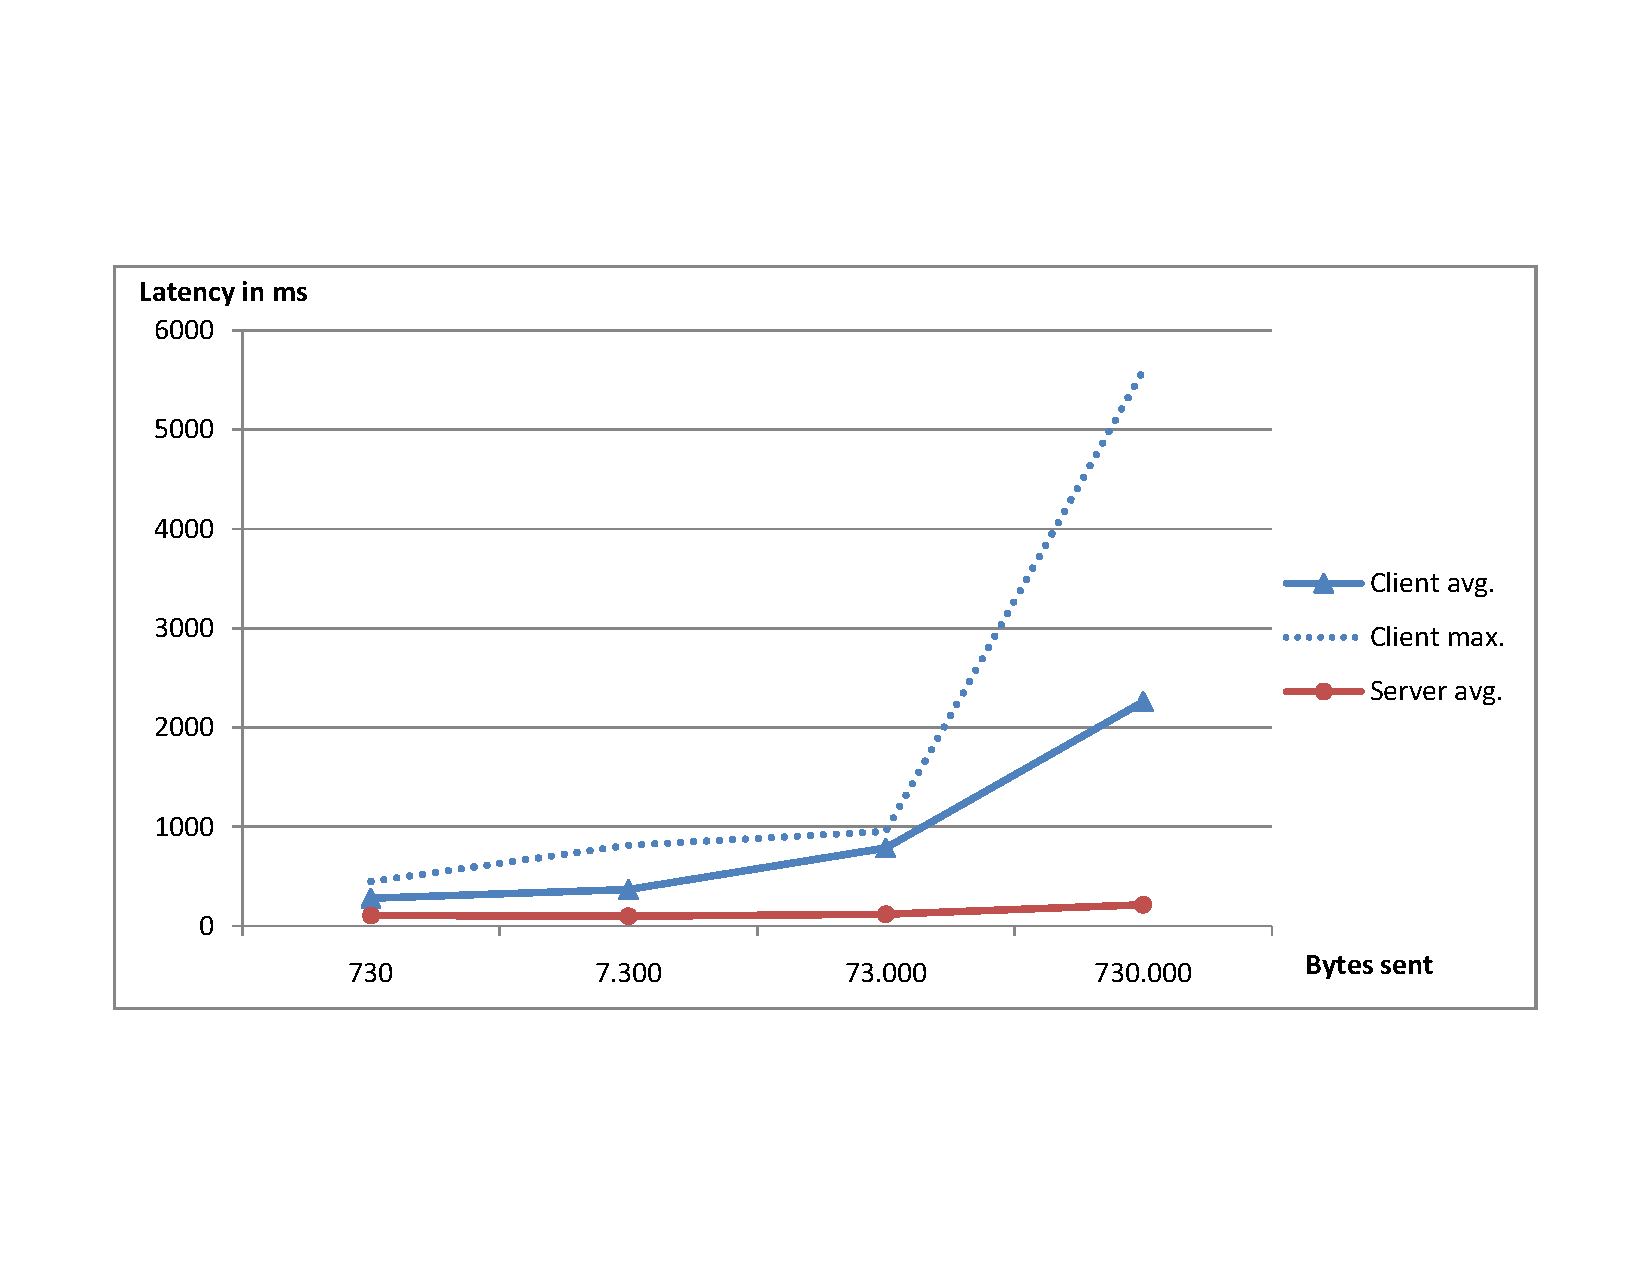
\includegraphics[trim = 0 5cm 0 5cm, width=10cm]{add_obj.pdf} 
	\caption{Adding Objects of Variable Size}
	\end{center}
	\end{figure}
}

\frame
{
	\frametitle{Add()}
	\begin{figure}[t]
	\begin{center}
	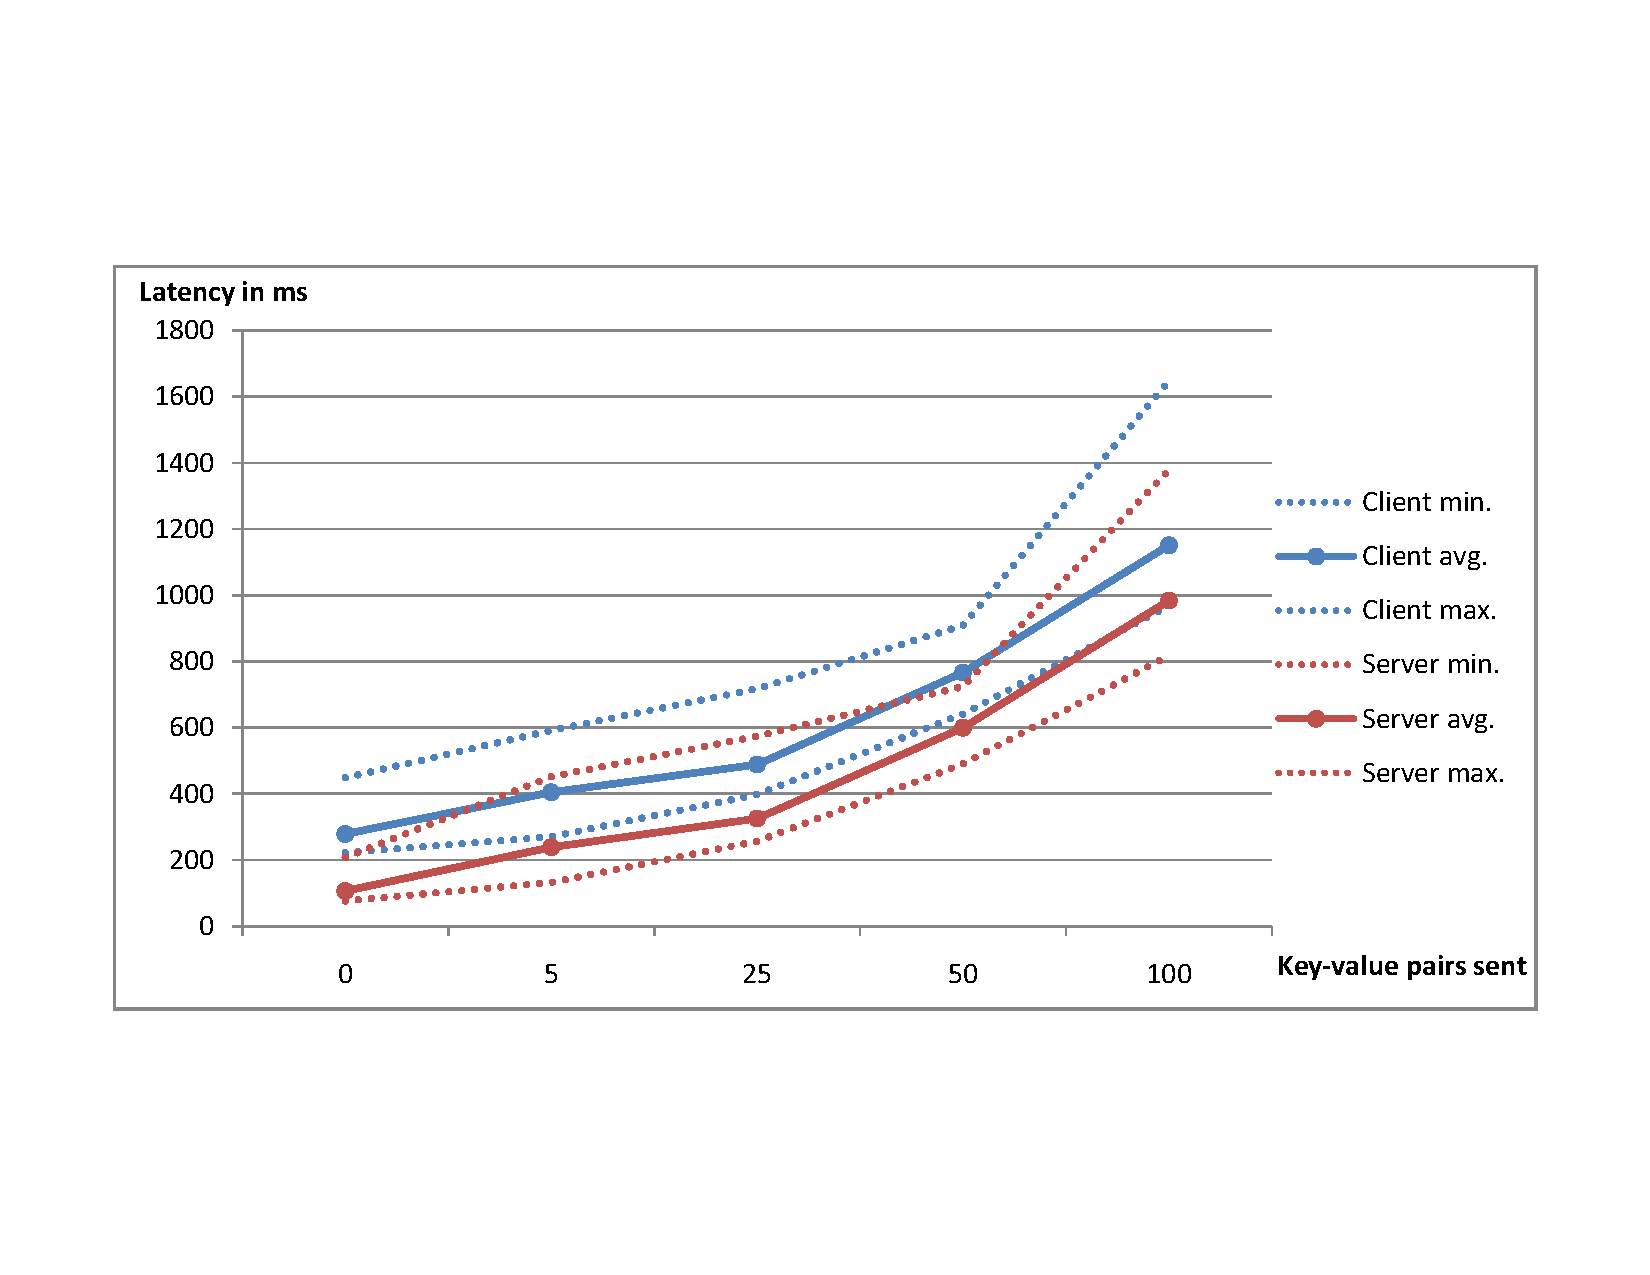
\includegraphics[trim = 0 5cm 0 5cm, width=10cm]{add_md.pdf} 
	\caption{Adding Objects with Variable Meta Data}
	\end{center}
	\end{figure}
}

\frame
{
	\frametitle{Get()}
	\begin{figure}[t]
	\begin{center}
	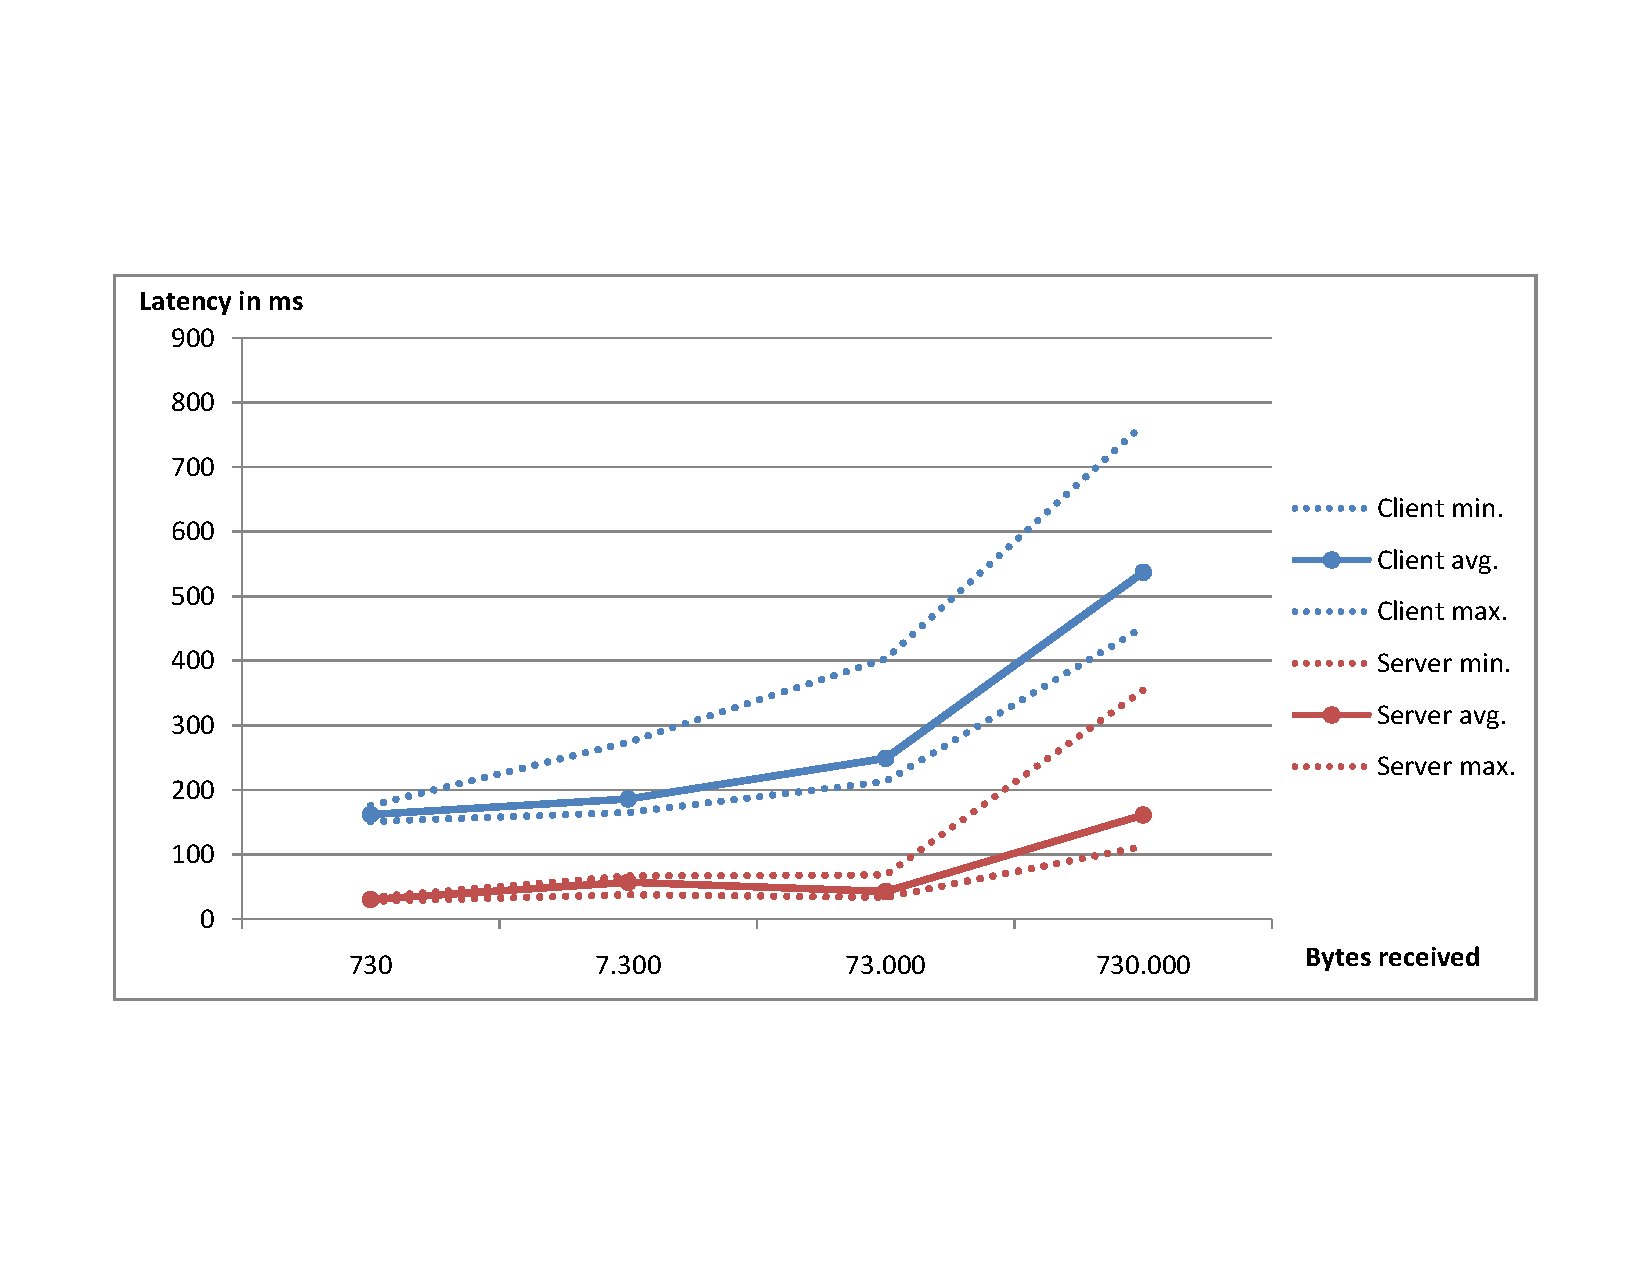
\includegraphics[trim = 0 5cm 0 5cm, width=10cm]{get_obj.pdf} 
	\caption{Retrieving Objects of Variable Size}
	\end{center}
	\end{figure}
}

\frame
{
	\frametitle{Get()}
	\begin{figure}[t]
	\begin{center}
	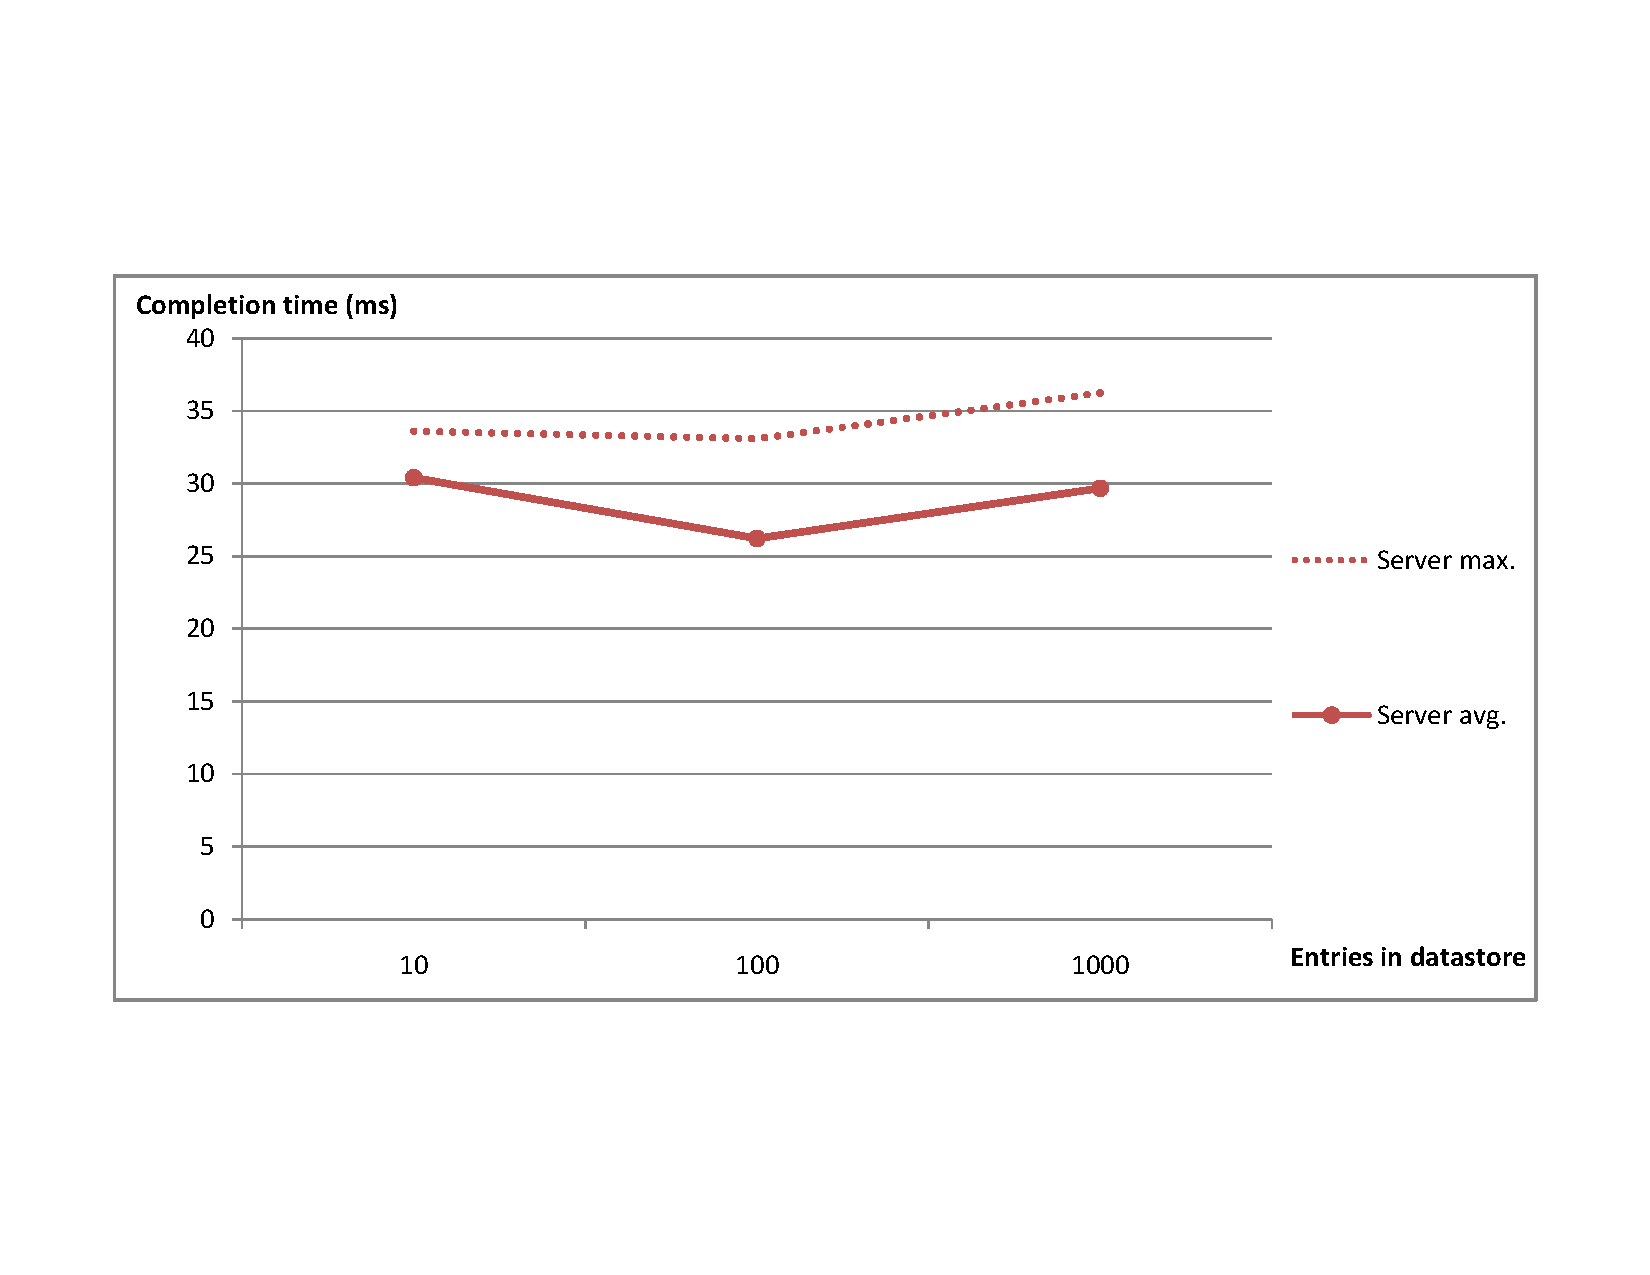
\includegraphics[trim = 0 5cm 0 5cm, width=10cm]{get_amt.pdf} 
	\caption{Retrieving Objects with Variable Meta Data}
	\end{center}
	\end{figure}
}

\frame
{
	\frametitle{Find()}
	\begin{figure}[t]
	\begin{center}
	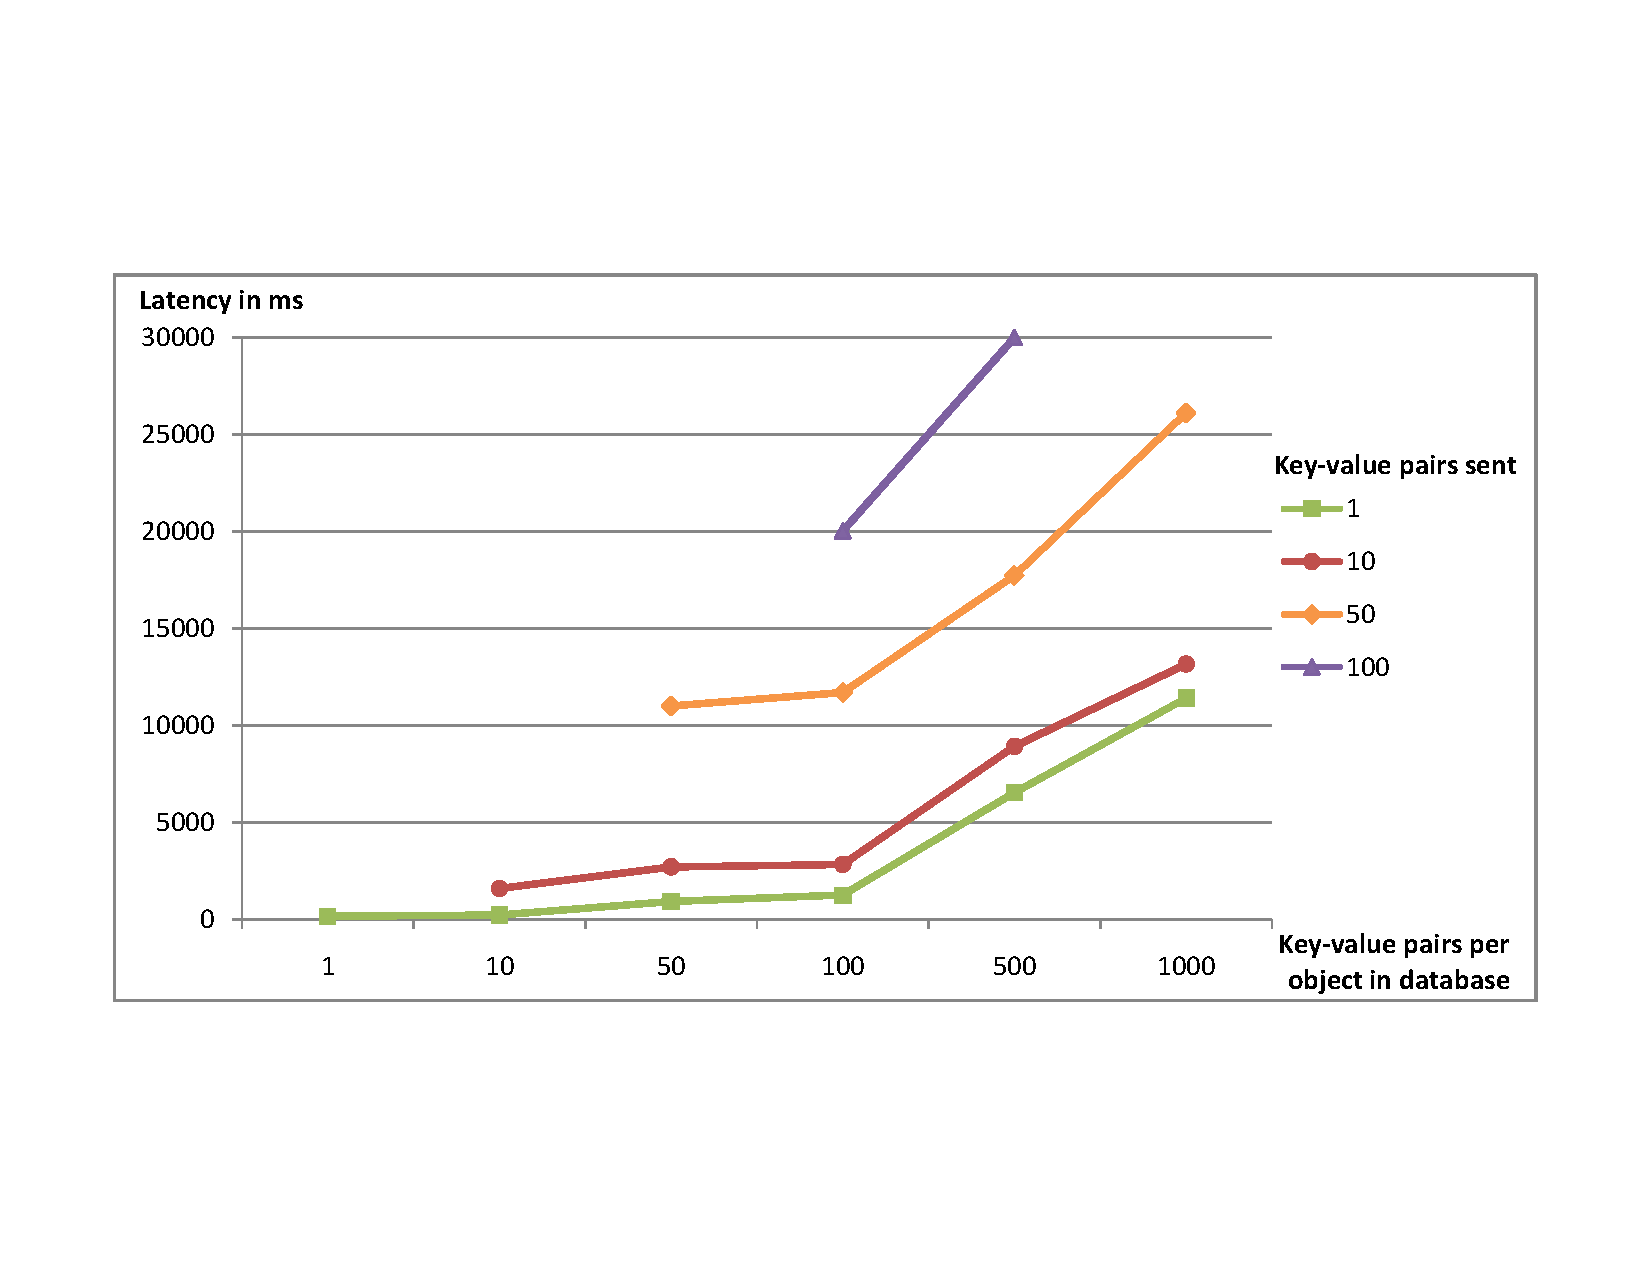
\includegraphics[trim = 0 5cm 0 5cm, width=10cm]{find_amt.pdf} 
	\caption{Finding Meta Data}
	\end{center}
	\end{figure}
}

\subsection{Clients in Parallel}
\frame
{
	\frametitle{Parellel Benchmarks}
	\textbf{TODO:} under construction!
}

\section{Applications}
\subsection{JavaGAT}
\frame
{
	\frametitle{JavaGAT}
	\begin{quote}
		JavaGAT offers a set of coordinated, generic and flexible APIs for accessing
		grid services from application codes, portals, data managements systems, etc.
	\end{quote}
	
	\begin{itemize}
		\item File operations (File, LogicalFile, RandomAccessFile, Endpoint)
		\item File stream operations (FileInputStream, FileOutputStream)
		\item Job submission (ResourceBroker)
		\item Monitoring (Monitorable)
		\item Access to information services (AdvertService)
	\end{itemize}
}

\frame[t]
{
	\frametitle{JavaGAT structure}
	\begin{figure}[t]
	\begin{center}
	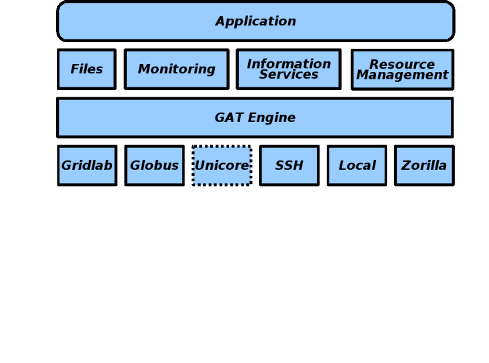
\includegraphics[width=8cm]{gat-design.png} 
	\end{center}
	\end{figure}
}

\frame[t]
{
	\frametitle{JavaGAT structure}
	\begin{figure}[t]
	\begin{center}
	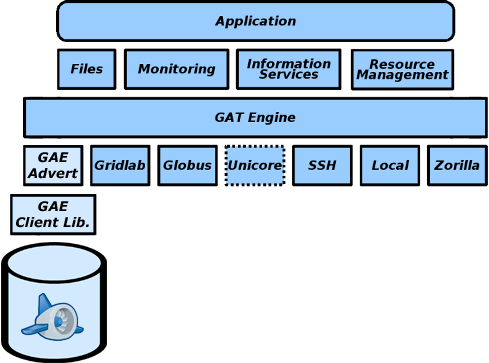
\includegraphics[width=8cm]{gat-mydesign.png} 
	\end{center}
	\end{figure}
}

\frame
{
	\frametitle{Our Solution}
	\begin{itemize}
		\item As of yet, only a local AdvertService existed
		\item Scalable design (local AdvertService does not scale)
		\item Completely transparent to user
		\item Path handling is done locally
    \end{itemize}
}

\subsection{IPL}
\frame
{
	\frametitle{IPL}
	\begin{quote}
		The IPL is a communication library is specifically designed for usage in a
		grid environment.
	\end{quote}
	\begin{figure}[h]
	\begin{center}
	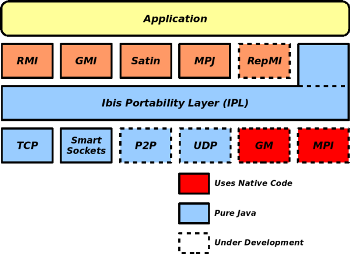
\includegraphics[width=5cm]{ibis-design.png} 
	\end{center}
	\end{figure}
}

\frame[t,containsverbatim]
{
	\frametitle{IPL Example}
	\begin{Verbatim}[fontsize=\small,gobble=2]
		$ $IPL_HOME/bin/ipl-server --events
		Ibis server running on 130.37.20.18-8888~bbn230
		List of Services:
		    Bootstrap service on virtual port 303
		    Central Registry service on virtual port 302
		    Management service
		Known hubs now: 130.37.20.18-8888~bbn230
		
		$IPL_HOME/bin/ipl-run \
		-Dibis.server.address=130.37.20.18-8888~bbn230 \
		-Dibis.pool.name=test \
		ibis.ipl.examples.Hello
    \end{Verbatim}
}

\frame[t,containsverbatim]
{
	\frametitle{IPL Example Using Advert Server (Server)}
	\begin{Verbatim}[fontsize=\small,gobble=2]
		$ $IPL_HOME/bin/ipl-server --events \
		--advert google://jondoe.appspot.com/identifier \
		--user jondoe@gmail.com --pass north23AZ \
		--metadata author=jondoe,created=24jun,pool=test,color=purple
		Ibis server running on 130.37.20.18-8888~bbn230
		List of Services:
		    Bootstrap service on virtual port 303
		    Central Registry service on virtual port 302
		    Management service
		Known hubs now: 130.37.20.18-8888~bbn230
	\end{Verbatim}
}

\frame[t,containsverbatim]
{
	\frametitle{IPL Example Using Advert Server (Application)}
	\begin{Verbatim}[fontsize=\small,gobble=2]
		$IPL_HOME/bin/ipl-run \
		-Dibis.advert.address=google://jondoe.appspot.com \
		-Dibis.advert.username=jondoe \
		-Dibis.advert.password=north23AZ \
		-Dibis.advert.metadata=created=24jun,color=purple \
		-Dibis.pool.name=test \
		ibis.ipl.examples.Hello
    \end{Verbatim}
}

\frame
{
	\frametitle{Our Solution}
	\begin{itemize}
    	\item No server for bootstrapping IPL registries existed
    	\item Large range of IPL registries can be started, whilst only rembering
    		one (advert) address
		\item Different groups of Ibis can be started without (manually) sharing the
			server address
    \end{itemize}
}

\section{Conclusion}
\subsection{Verdict}
\frame{
	\frametitle{Pros and Cons}
	Pros:
	\begin{itemize}
      \item[+] <1->Free of charge (until quota exceeds)
      \item[+] <1->Powerful engine and sufficient bandwidth
      \item[+] <1->Scalable design
      \item[+] <1->AdvertService only existed locally
      \item[+] <1->No registry bootstrap server existed, as of yet
    \end{itemize}
    
    \uncover<2->{Cons:}
    \begin{itemize}
      \item[-] <2->No guarantees
      \item[-] <2->Missing functionality in App Engine/Python
    \end{itemize}
}

\subsection{Questions}
\frame{
	\large{Any questions?}
}
\end{document}